\documentclass{article}[twocolumn]
\usepackage{tikz}
\usetikzlibrary{positioning}
\usetikzlibrary{external}
\tikzexternalize[prefix = fig/]
% \pgfrealjobname{overview}
\usepackage{float}

\title{COVIDetector}
\author{Andrea Tulimiero, Eshref Yozdemir, Peter Tatkowski}

\begin{document}
\maketitle

\section{Introduction}
\begin{figure}{h}
  \center
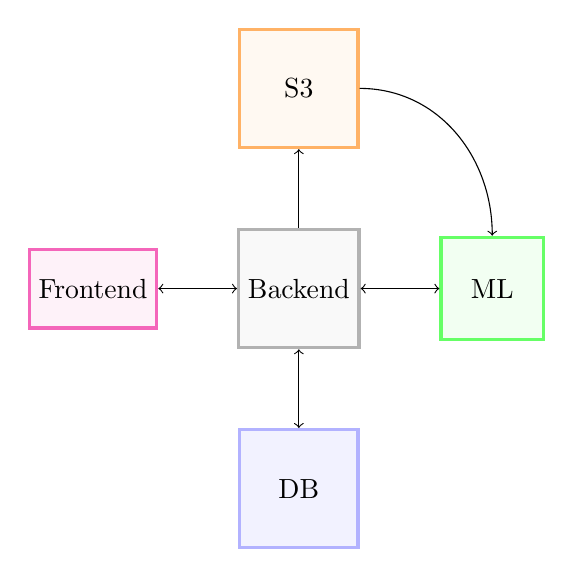
\begin{tikzpicture}[
frontnode/.style={rectangle, draw=magenta!60, fill=magenta!5, very thick, minimum size=10mm},
backnode/.style={rectangle, draw=gray!60, fill=gray!5, very thick, minimum size=15mm},
s3node/.style={rectangle, draw=orange!60, fill=orange!5, very thick, minimum size=15mm},
dbnode/.style={rectangle, draw=blue!30, fill=blue!5, very thick, minimum size=15mm},
mlnode/.style={rectangle, draw=green!60, fill=green!5, very thick, minimum size=13mm},
]
%Nodes
\node[frontnode]   (frontend)                     {Frontend};
\node[backnode]    (backend)  [right=of frontend] {Backend};
\node[s3node]      (s3)       [above=of backend]  {S3};
\node[dbnode]      (db)       [below=of backend]  {DB};
\node[mlnode]      (ml)       [right=of backend]  {ML};

%Lines
\draw[<->] (frontend.east) -- (backend.west);
\draw[->] (backend.north) -- (s3.south);
\draw[<->] (backend.south) -- (db.north);
\draw[<->] (backend.east) -- (ml.west);
\draw[->] (s3.east) .. controls +(right:10mm) and +(up:10mm) .. (ml.north);
\end{tikzpicture}
\label{fig:overview}
\caption{The overview of the project}
\end{figure}

\section{Frontend}

\section{Backend}
The backend is the component which receives sampling from the Frontend and give it to the ML model.
Moreover, it takes care of handling other tasks like registration and historical data management.

\subsection{Decoupling users from samples for anonymity}
When gathering users samples anonymity is paramount.
While realizing a decoupling system we wanted to keep most of the benefits of email verification and having a personal account, which are:
\begin{itemize}
  \item spam avoidance, thanks to email verification (and emails blacklisting) we can significantly reduce the amount of fake automated users that can register, and
  \item user samples history, which allows us to carry out also historical analysis to find out trends in changes due to the infection
\end{itemize}
To retain both these benefits we designed an anonymous token system.
The mechanism is depicted in figure \ref{fig:anon_token} and works as follows:
\begin{enumerate}
  \item The user specify its email and the frontend issues a registration request to the backend
  \item The backend sends an email to the user containing an activation link
  \item The frontend intercepts the activation link contained in the email, and
  \item issues a confirmation request to the backend
  \item The backend then completes the registration process by creating a patient account and returning an anonymous public and secret token to the application
\end{enumerate}
The \textit{secret} token is used to authenticate samples upload to avoid data skewing by malicious entities.
\begin{figure}[h]
  \centering
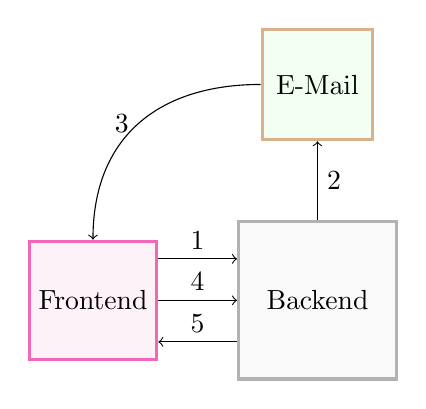
\begin{tikzpicture}[
frontnode/.style={rectangle, draw=magenta!60, fill=magenta!5, very thick, minimum size=15mm},
backnode/.style={rectangle, draw=gray!60, fill=gray!5, very thick, minimum size=20mm},
mailnode/.style={rectangle, draw=brown!60, fill=green!5, very thick, minimum size=14mm},
]
%Nodes
\node[frontnode]   (frontend)                     {Frontend};
\node[backnode]    (backend)  [right=of frontend] {Backend};
\node[mailnode]    (mail)     [above=of backend]  {E-Mail};

%Lines
\draw[->, transform canvas={yshift=15pt}] (frontend.east) -- (backend.west) node[midway, above] {1};
\draw[->] (backend.north) -- (mail.south) node[midway, right] {2};
\draw[->] (mail.west) .. controls +(left:13mm) and +(up:13mm) .. (frontend.north) node[midway, left] {3};
\draw[->, transform canvas={yshift=0pt}] (frontend.east) -- (backend.west) node[midway, above] {4};
\draw[<-, transform canvas={yshift=-15pt}] (frontend.east) -- (backend.west) node[midway, above] {5};
\end{tikzpicture}
\label{fig:anon_token}
\caption{The anonymous patient token system}
\end{figure}

\section{ML Model}
% TODO: Include sources
The Machine Learning model is highly based on the Reformer, which is a more memory-efficient version of the Transformer network. However, the raw audio sample itself is too large to fit into the model; therefore, we have to apply convolutions before the model is trained. Currently, three convolutional networks scale down the incoming audio file sample, so that the Transformer can process the audio file better. After it has been passed through this, further downsampling is performed, so that the model can output a classifier prediction.

Currently, this is how the model looks:

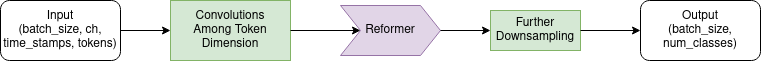
\includegraphics[width=1\textwidth]{fig/COVIDetector}

The input dimensions correspond to:
\begin{itemize}
    \item \texttt{batch\_size}: How many samples to train at once.
    \item \texttt{ch}: How many channels there are in the data. For \texttt{.wav} files, this corresponds to $1$.
    \item \texttt{time\_stamps}: The maximum amount of time samples a user can have. Each one corresponds to one predetermined interval of time.
    \item \texttt{tokens}: Each individual data reading of each audio sample.
\end{itemize}

The output dimensions correspond to this:
\begin{itemize}
    \item \texttt{batch\_size}: How many samples to train at once. Same as the input.
    \item \texttt{num\_classes}: How many classes to output.
\end{itemize}

% TODO: The following is an idea; can change later.
\texttt{num\_classes} will be the same size as \texttt{time\_stamps}; and each one of these will be a boolean as to whether or not the patient is sick on the time stamps in question.

For training, we are planning to mask out the two latest data samples, while still keeping the two target variables. That way, the model can learn whether or not the patient will get sick in the near future.

% TODO: Can add more information on training later...
\end{document}
